\def\mytitle{PYTHON PROGRAMMING ON MATRICES}
\def\myauthor{Revathi pamujula}
\def\contact{revathipamujula111@gmail.com}
\def\mymodule{Future Wireless Communication (FWC)}


\documentclass[10pt, a4paper]{article}
\usepackage[a4paper,outer=1.5cm,inner=1.5cm,top=1.75cm,bottom=1.5cm]{geometry}

\twocolumn
\usepackage{graphicx}
%\usepackage{karnaugh-map}
\usepackage{tabularx}
\usepackage{hyperref}
\usepackage[utf8]{inputenc}
\usepackage{amsmath}
%\usepackage{physics}
\usepackage{amssymb}
\usepackage{watermark}
\renewcommand*\familydefault{\sfdefault}
\usepackage{lipsum}
\usepackage{xcolor}
\usepackage{listings}
\let\vec\mathbf
\lstset{
frame=single, 
breaklines=true,
columns=fullflexible
}

\begin{document}
\title{\mytitle}
\author{\myauthor\hspace{1em}\\\contact\\FWC22045\hspace{6.5em}IITH\hspace{0.5em}\mymodule\hspace{6em}Matrix:Lines}

%\{ Wireless Communication (FWC)}
\date{}
\maketitle


  \section{Problem}
Find the angle between x-axis and the line joining points (3,-1) and (4,-2)

\section{Solution}
\textbf{Given that:}
\begin{center}

%\boldmath

$$\vec{P}=\begin{pmatrix} 3\\ -1\ \end{pmatrix}$$
$$\vec{Q}=\begin{pmatrix} 4\\ -2\ \end{pmatrix}$$
%\unboldmath
\end{center}
Finding the directive vector and assigning it to C\\
\begin{center}
%\boldmath
	$\vec{C}=\vec{P}-\vec{Q}$\\
%\unboldmath
\end{center}
\begin{center}
%\boldmath
	$\vec{C}=\begin{pmatrix} 3\\ -1\ \end{pmatrix} - \begin{pmatrix} 4\\ -2\ \end{pmatrix}$
%\unboldmath
\end{center}

\begin{center}
%\boldmath
$\vec{C}=\begin{pmatrix} -1\\ 1\ \end{pmatrix}$\\
%\unboldmath
\end{center}

  Now consider a vector (1,0) along x-axis and assign it to $x$\\
\begin{center}

%\boldmath
	$$\vec{x}=\begin{pmatrix} 1\\ 0\ \end{pmatrix}$$
%\unboldmath
\end{center}

By using the formula we can find the angle\\
\begin{center}
%\boldmath
	$cos\theta=\frac{\vec{C}^{T}\vec{X}}{||\vec{C}|| ||\vec{X}||}$\\
 %\unboldmath//
 $$\theta=135^{\circ}$$
 \end{center}
\begin{figure}[h!]
  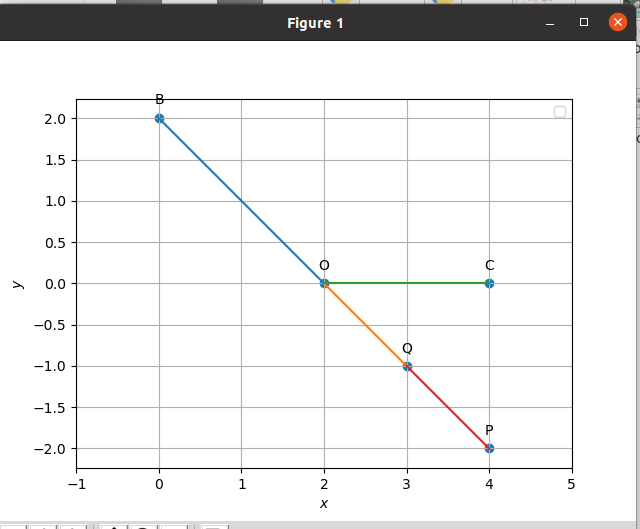
\includegraphics[scale=0.5]{fig.png}
  \caption{line assignment }
  \label{fig:line assignment}
\end{figure}
\end{document}
